% !TeX root = ../main.tex
% 原始章节：04-toolchain.Rmd

\chapter{数字电路设计训练}\label{chap:04-toolchain}

\section{LoongArch指令集32位精简版（LA32R）介绍}\label{sec:04-toolchain-001}

\subsection{指令集介绍}\label{sec:04-toolchain-002}

LoongArch是由龙芯中科自主研发的指令集架构，于2020年8月13日首次公开。其拥有基础指令、虚拟化扩展、二进制翻译扩展、向量扩展、高级向量扩展等
近2000条原生指令，具有完全自主、技术先进、兼容生态三方面特点。

LoongArch为32/64位定长RISC指令集，支持多种指令格式，针对MIPS、ARM、x86等指令集架构支持高效的二进制翻译。当前，LoongArch指令集生态日益
丰富，基础软件方面支持龙芯浏览器、Java、Node.js、Python、Ruby等；工具链方面支持GNU编译工具链、LLVM编译器、Golang编译器、Rust编译器等；
云计算方面支持Kubernetes、Docker等；系统软件方面，Linux主线已支持LoongArch 32/64。

LoongArch 32位精简版是LoongArch指令集的子集，其拥有基础指令140条，主要用于体系结构教学。LoongArch 32位精简版包含算术运算、移位运算、
转移、普通访存、原子访存、栅障、基础整数杂项、浮点运算类、浮点比较、浮点转换、浮点搬运、浮点分支、浮点普通访存、CSR访问、Cache维护、
TLB维护、特权杂项等17种指令类型。存储支持直接地址翻译和映射地址翻译两种模式，在映射地址翻译模式下，还可以通过直接映射配置窗口机制（DMW）
完成虚实地址的直接映射；存储访问支持一致可缓存和强序非缓存两种类型。LA32R与LoongArch 32/64的关系如图\ref{fig:la-branch}所示。

\begin{figure}[htbp]
  \centering
  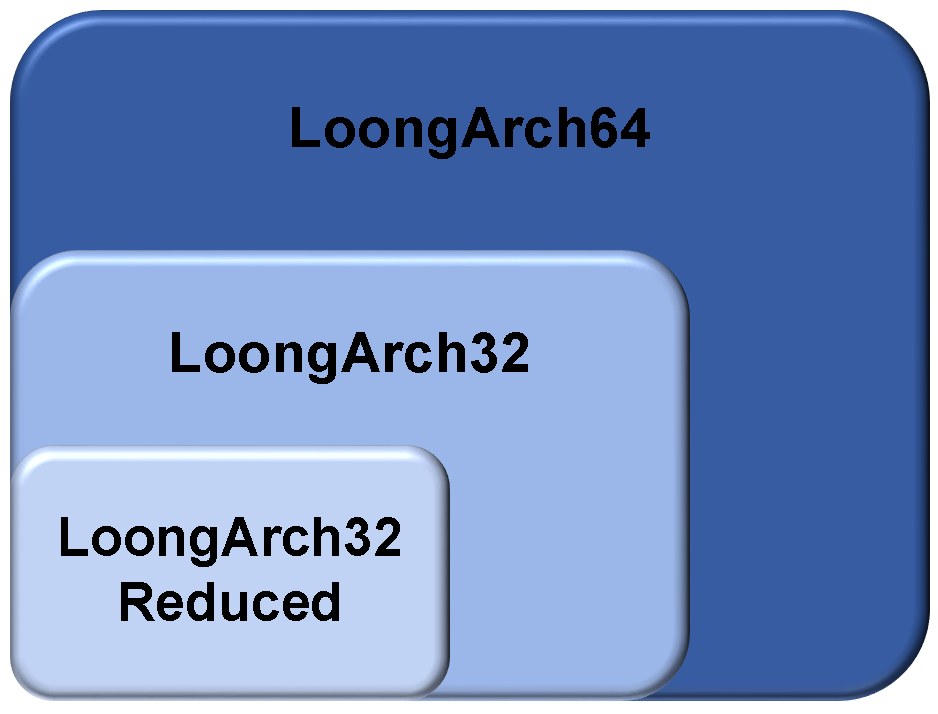
\includegraphics[width=0.5\linewidth]{assets/04/la-branch.png}
  \caption{龙架构的三个分支}
  \label{fig:la-branch}
\end{figure}

LoongArch 32位精简版支持例外和中断。中断采用线中断形式，每个处理器核内部可记录12个线中断，包括1个核间中断（IPI）、1个定时器中断（TI）、
8个硬中断（HWI0～HWI7）、2个软中断（SWI0～SWI1）。所有的线中断都是电平中断，且都是高电平有效。

例外包含中断（INT）、load操作页无效（PIL）、store操作页无效（PIS）、取指操作页无效（PIF）、页修改（PME）、页特权等级不合规（PPI）、
取指地址错（ADEF）、访存指令地址错（ADEM）、地址非对齐（ALE）、系统调用（SYS）、断点（BRK）、指令不存在（INE）、指令特权等级错（IPE）、
浮点指令未使能（FPD）、基础浮点指令例外（FPE）、TLB重填（TLBR）等16种例外。

龙架构具有较好的自主性、先进性与兼容性。龙架构从整个架构的顶层规划，到各部分的功能定义，再到细节上每条指令的编码、名称、含义，在架构上进行自主重新设计，
具有充分的自主性。龙架构摒弃了传统指令系统中部分不适应当前软硬件设计技术发展趋势的陈旧内容，吸纳了近年来指令系统设计领域诸多先进的技术发展成果。
同原有兼容指令系统相比，不仅在硬件方面更易于高性能低功耗设计，而且在软件方面更易于编译优化和操作系统、虚拟机的开发。

\subsection{指令编码格式}\label{sec:04-toolchain-003}

龙芯架构32位精简版中的所有指令均采用32位固定长度，且指令的地址都要求4字节边界对齐。当指令地址不对齐时将触发地址错例外。

指令编码的风格是所有寄存器操作数域都从第0比特开始从低到高依次摆放。操作码都是从第31比特开始从高到低依次摆放。如果指令中包含有立即数操作数，那么立即数域位于寄存器域和操作码域之间，根据不同指令类型有不同的长度。

具体来说,包含9种典型的指令编码格式,即3种不含立即数的编码格式2R、3R、4R,以及6种含立即数的编码格式2RI8、2RI12、2RI14、2RI16、1RI21、I26。表1-1列举了这9种典型编码格式的具体定义。

需要指出的是,存在少数指令,其指令编码域并不完全等同于这9种典型指令编码格式,而是在其基础上略有变化。不过这种指令的数目并不多,且变化的幅度也不大,不会对于编译系统的开发人员带来不便。

9种典型指令编码格式的定义如图\ref{fig:encoding-format}所示。

\begin{figure}[htbp]
  \centering
  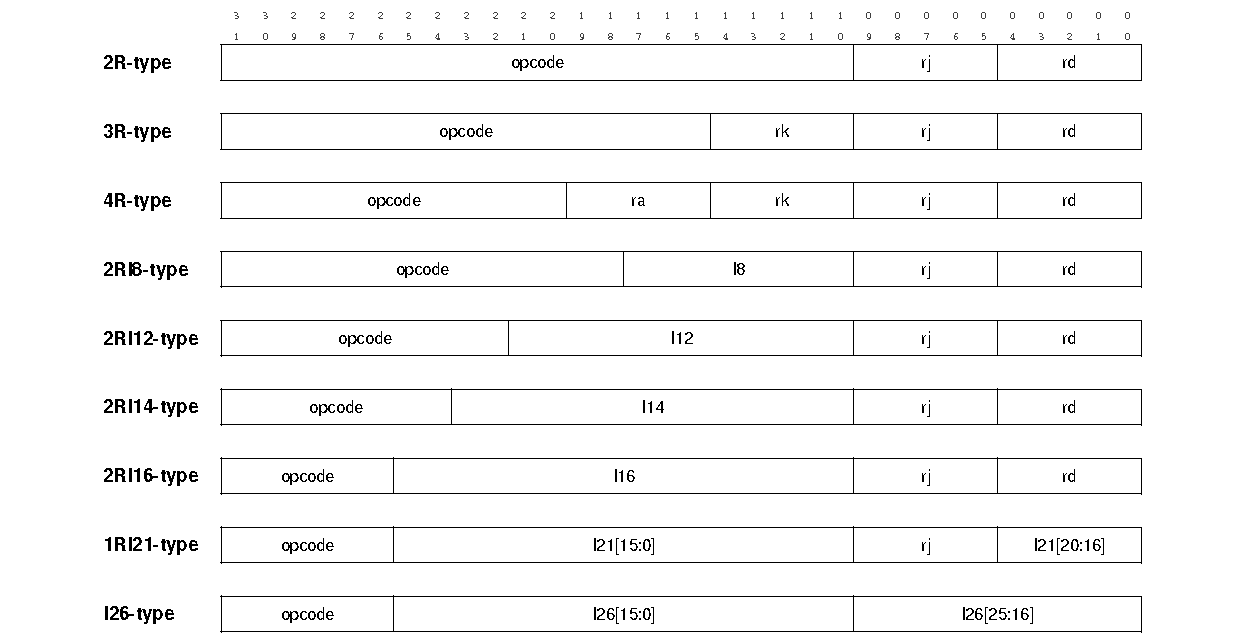
\includegraphics[width=1\linewidth]{assets/04/encoding-format.pdf}
  \caption{LA32R指令编码格式}
  \label{fig:encoding-format}
\end{figure}

\subsection{指令分类}\label{sec:04-toolchain-004}

LA32R指令集的指令类型可以分为以下几类：

\begin{itemize}
\item \textbf{整数分支跳转指令}：用于控制程序流的跳转和分支。
\item \textbf{整数计算指令}：用于进行各种整数运算。
\item \textbf{整数访存指令}：用于内存的读取和写入。
\item \textbf{特权指令集}：包括操作系统和硬件特权操作的指令。
\item \textbf{浮点指令集}：虽然本节不展开详细介绍，但浮点指令集包括用于浮点运算的指令。
\end{itemize}


\subsection{指令助记符}\label{sec:04-toolchain-005}

在龙芯架构的32位精简版中，指令汇编助记格式主要包括指令名和操作数两部分，为方便汇编编程人员和编译器开发人员使用，采用了统一的前、后缀规则。

\begin{enumerate}
\def\labelenumi{\arabic{enumi}.}
\tightlist
\item
  \textbf{指令名前缀}：

  \begin{itemize}
  \tightlist
  \item
    所有非向量浮点数指令的指令名以字母``F''开头，以区分整数和浮点数指令。
  \end{itemize}
\item
  \textbf{指令名后缀}：

  \begin{itemize}
  \tightlist
  \item
    绝大多数指令通过``.XX''形式的后缀来指示指令的操作对象类型。
  \item
    整数类型操作对象的后缀：

    \begin{itemize}
    \tightlist
    \item
      \texttt{.B}：有符号字节
    \item
      \texttt{.H}：有符号半字
    \item
      \texttt{.W}：有符号字
    \item
      \texttt{.BU}：无符号字节
    \item
      \texttt{.HU}：无符号半字
    \item
      \texttt{.WU}：无符号字
    \item
      注意：当操作数是否有符号不影响运算结果时，后缀不带``U''。
    \end{itemize}
  \item
    浮点数类型操作对象的后缀：

    \begin{itemize}
    \tightlist
    \item
      \texttt{.H}：半精度浮点数
    \item
      \texttt{.S}：单精度浮点数
    \item
      \texttt{.D}：双精度浮点数
    \item
      \texttt{.W}：有符号字
    \item
      \texttt{.WU}：无符号字
    \end{itemize}
  \end{itemize}
\item
  \textbf{无后缀情况}：

  \begin{itemize}
  \tightlist
  \item
    某些指令的操作对象数据位宽由处理器的实现（32位或64位）决定，例如SLT和SLTU指令。
  \item
    特权态指令（操作CSR、TLB和Cache）以及在不同寄存器文件之间移动数据的指令也不加后缀。
  \end{itemize}
\item
  \textbf{后缀组合}：

  \begin{itemize}
  \tightlist
  \item
    当源操作数和目的操作数的数据位宽和有无符号情况一致时，指令名只有一个后缀。
  \item
    如果源操作数数据位宽和有无符号情况一致，但与目的操作数不一致，指令名有两个后缀，第一个后缀表示目的操作数，第二个后缀表示源操作数。
  \item
    若源操作和目的操作数情况更复杂，指令名将按顺序列出目的操作数和每个源操作数的情况。
  \end{itemize}

  例如：

  \begin{itemize}
  \tightlist
  \item
    指令``MULW.D.WU rd, rj, rk''中：

    \begin{itemize}
    \tightlist
    \item
      \texttt{.D}对应目的操作数\texttt{rd}
    \item
      \texttt{.WU}对应源操作数\texttt{rj}和\texttt{rk}
    \item
      表示该乘法指令将两个无符号字相乘，结果是双字，写入\texttt{rd}中。
    \end{itemize}
  \item
    指令``CRC.W.B.W rd, rj, rk''中：

    \begin{itemize}
    \tightlist
    \item
      第一个\texttt{.W}对应\texttt{rd}
    \item
      \texttt{.B}对应\texttt{rj}
    \item
      第二个\texttt{.W}对应\texttt{rk}
    \item
      表示该CRC校验指令将\texttt{rj}中的字节消息与\texttt{rk}中的32位原校验值生成新的32位校验值，结果写入\texttt{rd}中。
    \end{itemize}
  \end{itemize}
\item
  \textbf{寄存器操作数}：

  \begin{itemize}
  \tightlist
  \item
    通用寄存器使用``rN''表示，其中N为寄存器编号。
  \item
    浮点寄存器使用``fN''表示，其中N为寄存器编号。
  \end{itemize}
\end{enumerate}

\section{LA32R指令集与MIPS指令集对比}\label{sec:04-toolchain-006}

\subsection{编码格式对比}\label{sec:04-toolchain-007}

LA32R与MIPS指令集（MIPS R4K）均为经典的RISC风格指令集，具有固定长度的指令格式。两者的编码格式存在一定差异。LA32R指令集采用了更丰富和清晰的指令编码格式，并且使用了前缀编码的技术。这使得LA32R在编码简洁性和灵活性方面优于MIPS。

\subsection{4.2.2 整数指令对比}\label{sec:04-toolchain-008}

在整数指令方面，LA32R相较于MIPS指令集有所简化。例如，LA32R没有HI/LO寄存器，也没有CLO/CLZ指令。LA32R还省略了xWL/xWR非对齐字访存指令。此外，LA32R的分支跳转指令没有延迟槽，并且立即数长度更长，使得跳转指令的执行更加高效和简洁。

\subsection{4.2.3 特权指令对比}\label{sec:04-toolchain-009}

在特权指令方面，LA32R与MIPS指令集有显著不同。LA32R在内存管理方面支持窗口映射和直接映射的机制，而MIPS则采用了固定窗口映射。LA32R简化了中断异常处理流程，并且在hazard控制方面相比MIPS进行了简化，使得处理器设计和实现更加高效。

\section{LA32R处理器开发工具流程}\label{sec:04-toolchain-010}

\subsection{Chiplab 验证环境介绍}\label{sec:04-toolchain-011}

chiplab项目是由龙芯提出，用于构建LA32R SoC的敏捷开发平台。其chip文件夹包含仿真/FPGA三套顶层SoC，IP文件夹放置SoC使用到的IP，包含处理器、SPI、Confreg等。

仿真的工作目录位于sims/verilator/run\_*，当前仅支持verilator。run\_prog : 该工作目录下可运行func测试用例、dhrystone、coremark性能测试程序、linux以及自定义C程序。run\_random : 该工作目录下可进行随机指令序列测试。

综合工作目录位于fpga，当前支持龙芯实验箱及百芯开发板。使用vivado打开loongson/20*.2/system\_run.xpr（根据具体vivado版本选择）或者Baixin/system\_run/system\_run.xpr工程文件，添加处理器核代码后，可直接开始综合。若选择添加chiplab中的参考核，注意添加myCPU/IP下的xilinx IP。
处理器核输入时钟频率默认为33MHz，可对clk\_pll\_33xilinx IP的输出时钟频率进行调整，修改处理器核的输入时钟频率。此外，还需将chip/soc\_demo/loongson/config.h或者chip/soc\_demo/Baixin/config.h文件中的FREQ宏定义修改为对应频率。

\subsection{Eula-Env 验证环境介绍}\label{sec:04-toolchain-012}

Eula-Env 项目是由北航百芯团队提供，致力于构建 LoongArch 32 Reduced 集成芯片敏捷开发平台，提供了全面的设计和测试框架。本节将介绍 Eula-Env 的功能。

Eula-Env 的文件结构如下：

\begin{itemize}
\tightlist
\item
  \texttt{am/}: 基于南京大学 AM 移植的 LoongArch 32 Reduced 裸机运行时环境
\end{itemize}

\begin{quote}
原仓库地址: \url{https://github.com/NJU-ProjectN/abstract-machine.git}
\end{quote}

\begin{itemize}
\item
  \texttt{eulacore}: 基于敏捷开发平台设计实现的九级顺序单发射处理器与 Verilator 仿真 SoC
\item
  \texttt{la32r-toolchains}: LoongArch 32 Reduced GNU 工具链和 newlib 链接库
\item
  \texttt{nemu}: 基于南京大学 NEMU 移植的 LoongArch 32 Reduced 仿真模拟器
\end{itemize}

\begin{quote}
原仓库地址: \url{https://gitee.com/wwt_panache/la32r-nemu.git}
\end{quote}

\begin{itemize}
\item
  \texttt{env.sh}: 环境变量加载脚本，需在编译程序前使用
\item
  \texttt{setup-tools.sh}: 依赖库/工具安装脚本
\item
  \texttt{setup.sh}: 一键配置脚本, 包含 env.sh 的功能, 初始化仓库子模块，并自动编译 nemu 与 am 中的 coremark 程序
\end{itemize}

通过 \texttt{setup.sh} 脚本，我们可以一键加载环境变量/编译 NEMU/编译 AM 的 Coremark 程序，而根据实际需求，我们可以逐一进行如下操作。

\begin{enumerate}
\def\labelenumi{\arabic{enumi}.}
\tightlist
\item
  加载环境变量
\end{enumerate}

% 代码语言：BookShell
\begin{CodeBlock}[language=BookShell]
$ source env.sh
\end{CodeBlock}

\begin{enumerate}
\def\labelenumi{\arabic{enumi}.}
\setcounter{enumi}{1}
\tightlist
\item
  编译行为仿真模型
\end{enumerate}

针对 CPU 设计的早期阶段，该项目设计了一套简易的 Verialtor 仿真 SoC，CPU 对外统一为一个 AXI4 接口，并通过 AXI4 转接桥连接 RAM、UART8250、Confreg，CPU具体定义如下图所示：

% 代码语言：BookVerilog
\begin{CodeBlock}[language=BookVerilog]
module mycpu_mega_top(
  input         clock,
  input         reset,
  input         awready,
  output        awvalid,
  output [31:0] awaddr,
  output [2:0]  awprot,
  output        awid,
  output        awuser,
  output [7:0]  awlen,
  output [2:0]  awsize,
  output [1:0]  awburst,
  output        awlock,
  output [3:0]  awcache,
  output [3:0]  awqos,
  input         wready,
  output        wvalid,
  output [31:0] wdata,
  output [3:0]  wstrb,
  output        wlast,
  output        bready,
  input         bvalid,
  input  [1:0]  bresp,
  input         bid,
  input         buser,
  input         arready,
  output        arvalid,
  output [31:0] araddr,
  output [2:0]  arprot,
  output        arid,
  output        aruser,
  output [7:0]  arlen,
  output [2:0]  arsize,
  output [1:0]  arburst,
  output        arlock,
  output [3:0]  arcache,
  output [3:0]  arqos,
  output        rready,
  input         rvalid,
  input  [1:0]  rresp,
  input  [31:0] rdata,
  input         rlast,
  input         rid,
  input         ruser,
  input  [7:0]  ext_int,
  output        global_reset
);
\end{CodeBlock}

为使得 CPU 接入该项目的 SoC，首先需要通过如下命令编译 SoC 仿真顶层模块，生成 SimTop.v 文件:

% 代码语言：BookShell
\begin{CodeBlock}[language=BookShell]
$ make verilog
\end{CodeBlock}

可以看到 SimTop.v 中包含了该项目的 SoC 顶层并实例化了 CPU 模块:

% 代码语言：BookVerilog
\begin{CodeBlock}[language=BookVerilog]
mycpu_mega_top core ( // @[EulaSimTop.scala 27:20]
   .awready(core_awready),
   .awvalid(core_awvalid),
   ...
   .rready(core_rready),
   .rvalid(core_rvalid),
   .rresp(core_rresp),
   .rdata(core_rdata),
   .rlast(core_rlast),
   .rid(core_rid),
   .ruser(core_ruser),
   .ext_int(core_ext_int),
   .clock(core_clock),
   .reset(core_reset),
   .global_reset(core_global_reset)
 );
\end{CodeBlock}

然而，SimTop.v 中并没有对应 CPU 的实现部分，这部分需要使用者进行添加：将 CPU 顶层命名为 \texttt{mycpu\_mega\_top}, 并使其对外为一个 AXI 4 接口，具体接口定义如前面所示。假设 CPU 顶层模块文件名为 core.v (例如文件路径为 eula-env/eulacore/core.v，其中需要哦包含 CPU 顶层模块 \texttt{mycpu\_mega\_top})，最后在 SimTop.v 第一行引入 core.v 文件的路径

% 代码语言：BookVerilog
\begin{CodeBlock}[language=BookVerilog]
`include "../core.v" // 使用者根据自身 CPU 顶层模块文件路径添加

module AXI4RAM(
  input         clock,
  input         reset,
  ...
);
\end{CodeBlock}

完成上述步骤后，在 eula-env/eulacore 目录输入:

% 代码语言：BookShell
\begin{CodeBlock}[language=BookShell]
$ make emu EMU_TRACE=1 # 若不需要导出波形，可以不添加 EMU_TRACE=1 参数
\end{CodeBlock}

即可将 SimTop.v 与使用者的 CPU 共同编译为 C++ 行为模型，编译产物为 eula-env/eulacore/build/emu。

\begin{enumerate}
\def\labelenumi{\arabic{enumi}.}
\setcounter{enumi}{2}
\tightlist
\item
  编译 NEMU
\end{enumerate}

% 代码语言：BookShell
\begin{CodeBlock}[language=BookShell]
$ cd ${NEMU_HOME}
$ make la32-reduced-ref_defconfig
make -j
\end{CodeBlock}

\begin{enumerate}
\def\labelenumi{\arabic{enumi}.}
\setcounter{enumi}{3}
\tightlist
\item
  编译 AM
\end{enumerate}

以 coremark 程序为例

% 代码语言：BookShell
\begin{CodeBlock}[language=BookShell]
$ cd ${AM_HOME}/apps/coremark
$ make ARCH=la32r-eula
\end{CodeBlock}

\begin{enumerate}
\def\labelenumi{\arabic{enumi}.}
\setcounter{enumi}{4}
\tightlist
\item
  运行仿真测试
\end{enumerate}

% 代码语言：BookShell
\begin{CodeBlock}[language=BookShell]
$ cd ${PROJECT_ROOT}/eulacore/build
$ ./emu -i ${AM_HOME}/apps/coremark/build/coremark-la32r-eula.bin

# 如需导出波形，可添加 --dump-wave --wave-path="<your wave path>" 参数，注意前提是在编译 emu 的时候已经添加了 EMU_TRACE=1 参数
# 如需控制导出波形的周期，可添加 -b <begin cycle> -e <env cycle> 参数
\end{CodeBlock}

\begin{enumerate}
\def\labelenumi{\arabic{enumi}.}
\setcounter{enumi}{5}
\tightlist
\item
  查看波形
\end{enumerate}

% 代码语言：BookShell
\begin{CodeBlock}[language=BookShell]
$ gtkwave "<your wave path>"
\end{CodeBlock}

\subsection{LA32R-QEMU}\label{sec:04-toolchain-013}

QEMU（Quick EMUlator）是一个开源的虚拟机监控器和全系统模拟器，可以运行在多种主机平台上（如Linux、Windows、macOS等）。其具有如下功能：

\begin{itemize}
\item
  虚拟化技术：QEMU支持硬件虚拟化和软件虚拟化，可以模拟多种处理器架构（如x86、ARM、RISC-V等）。
\item
  系统仿真：QEMU能够模拟完整的计算机系统，包括处理器、存储、网络设备等，使得用户能够在一个平台上运行不同的操作系统和软件。
\end{itemize}

龙芯公司基于QEMU主线开发了支持LA32R指令集架构的版本，可见\url{https://gitee.com/loongson-edu/la32r-QEMU}

\subsection{整体流程介绍}\label{sec:04-toolchain-014}

从处理器核心设计开始，经过Chiplab中的对拍仿真测试，到使用Vivado进行上版验证，最后移植适配Linux。这一系列的步骤形成了LA32R处理器的开发流程。我们将详细介绍每一步的具体过程和注意事项。

为了开发一个LA32R处理器，我们推荐读者使用Eula-Env平台，可见 \url{https://github.com/BUAA-CI-LAB/eula-env}。处理器设计完成后，你可以通过如下步骤接入Eula-Env平台的DiffTest差分测试框架。

\begin{enumerate}
\def\labelenumi{\arabic{enumi}.}
\item
  处理器内部实例化 Difftest* 模块并连线；
\item
  处理器内部实例化 Difftest* 模块并连线；
\item
  仿真顶层和 difftest 共同编译为 C++ 行为模型 emu，emu 可运行由 AM 编译生成的裸机程序并进行差分测试。
\end{enumerate}

对于上板验证，读者可以直接打开\url{https://github.com/BUAA-CI-LAB/MegaSoC}仓库的Vivado工程文件，并导入CPU文件，更新IP核后，即可进行综合和实现。其中，CPU顶层如图所示：

% 代码语言：BookVerilog
\begin{CodeBlock}[language=BookVerilog]
module mycpu_mega_top(
  input         clock,
  input         reset,
  input         awready,
  output        awvalid,
  output [31:0] awaddr,
  output [2:0]  awprot,
  output        awid,
  output        awuser,
  output [7:0]  awlen,
  output [2:0]  awsize,
  output [1:0]  awburst,
  output        awlock,
  output [3:0]  awcache,
  output [3:0]  awqos,
  input         wready,
  output        wvalid,
  output [31:0] wdata,
  output [3:0]  wstrb,
  output        wlast,
  output        bready,
  input         bvalid,
  input  [1:0]  bresp,
  input         bid,
  input         buser,
  input         arready,
  output        arvalid,
  output [31:0] araddr,
  output [2:0]  arprot,
  output        arid,
  output        aruser,
  output [7:0]  arlen,
  output [2:0]  arsize,
  output [1:0]  arburst,
  output        arlock,
  output [3:0]  arcache,
  output [3:0]  arqos,
  output        rready,
  input         rvalid,
  input  [1:0]  rresp,
  input  [31:0] rdata,
  input         rlast,
  input         rid,
  input         ruser,
  input  [7:0]  ext_int,
  output        global_reset
);
\end{CodeBlock}

生成Bit流文件后，将开发板与主机间的下载线连接好，开发板上电，使用 Vavidao 工具里的 Open Hardware Manager 下载 Bit 文件到开发板上即可。

\section{LA32R系统支持与调试方法}\label{sec:04-toolchain-015}

\subsection{Uboot 介绍}\label{sec:04-toolchain-016}

Uboot是一个开源的Bootloader，主要用于嵌入式系统中，负责在硬件启动后初始化系统硬件设备并引导操作系统。
在硬件启动时执行，Uboot负责初始化 CPU、内存、外设等硬件设备，能够加载并引导各种文件系统格式，如 ext2/3/4, FAT，并提供命令行交互界面，允许用户执行各种操作，如引导系统、修改系统配置等。
其支持多种编译选项和配置，可以根据具体需求进行定制和扩展。

其目录结构如下：

\begin{itemize}
\item
  /arch 架构特定的文件

  \begin{enumerate}
  \def\labelenumi{\arabic{enumi}.}
  \item
    /arc 适用于ARC架构的通用文件
  \item
    /arm 适用于ARM架构的通用文件
  \item
    /m68k 适用于m68k架构的通用文件
  \item
    /microblaze 适用于microblaze架构的通用文件
  \item
    /mips 适用于MIPS架构的通用文件
  \item
    /nds32 适用于NDS32架构的通用文件
  \item
    /nios2 适用于Altera NIOS2架构的通用文件
  \item
    /powerpc 适用于PowerPC架构的通用文件
  \item
    /riscv 适用于RISC-V架构的通用文件
  \item
    /sandbox 适用于硬件无关的''沙盒''环境的通用文件
  \item
    /sh 适用于SH架构的通用文件
  \item
    /x86 适用于x86架构的通用文件
  \item
    /xtensa 适用于Xtensa架构的通用文件
  \end{enumerate}
\item
  /api 机器/架构无关的外部应用程序API
\item
  /board 版本相关的文件
\item
  /boot 镜像和引导支持
\item
  /cmd U-Boot命令函数
\item
  /common 各种架构无关的函数
\item
  /configs 板子默认配置文件
\item
  /disk 磁盘驱动分区处理代码
\item
  /doc 文档（包含ReST和README）
\item
  /drivers 设备驱动程序
\item
  /dts 用于构建内部 U-Boot fdt 的 Makefile
\item
  /env 环境支持
\item
  /examples 独立应用程序示例代码等
\item
  /fs 文件系统代码（cramfs, ext2, jffs2等）
\item
  /include 头文件
\item
  /lib 各架构通用的库函数
\item
  /Licenses 各种许可证文件
\item
  /net 网络代码
\item
  /post 上电自检
\item
  /scripts 各种构建脚本和Makefile
\item
  /test 各种单元测试文件
\item
  /tools 用于构建和签名 FIT 镜像等的工具
\end{itemize}

通过如下命令，你可以构建LA32R架构的Uboot：

% 代码语言：BookShell
\begin{CodeBlock}[language=BookShell]
$ export DEVICE_TREE=la32rmega_demo;
$ export ARCH=la32r;
$ export CROSS_COMPILE=loongarch32r-linux-gnusf-;
$ clear && make la32rmega_defconfig && make -j && loongarch32r-linux-gnusf-objdump -S u-boot > u-boot.S;
$ loongarch32r-linux-gnusf-objcopy ./u-boot -O binary u-boot.bin
\end{CodeBlock}

\subsection{Linux 介绍}\label{sec:04-toolchain-017}

Linux 是一个开源的类 Unix 操作系统内核，广泛应用于计算机系统、服务器和嵌入式设备。

通过如下命令，你可以构建LA32R架构的Linux：

% 代码语言：BookShell
\begin{CodeBlock}[language=BookShell]
export ARCH=loongarch;
export CROSS_COMPILE=loongarch32r-linux-gnusf-;
clear && make la32rmega_defconfig && make -j nproc
\end{CodeBlock}

\subsection{Linux 移植}\label{sec:04-toolchain-018}

Linux移植包括多个级别的工作：体系结构级别、SoC级别和板级。我们将以MegaSoC为例，重点介绍SoC级别上的移植工作，说明如何在Linux中添加相应的设备树支持。

首先在\texttt{linux/arch/loongarch/boot/dts/loongson}文件夹添加\texttt{la32rmega\_demo.dts}文件：

% 代码语言：BookDTS
\begin{CodeBlock}[language=BookDTS]
/dts-v1/;
/{
    model = "loongson,generic";
    compatible = "loongson,loongson3";
    #address-cells = <1>;
    #size-cells = <1>;

    aliases {
        serial0 = &cpu_uart0;
        mmc0 = &mmc0;
    };

    chosen {
        stdout-path = "serial0:230400n8";
        bootargs = "earlycon";
        ranges;
        framebuffer: framebuffer@7800000 {
            compatible = "simple-framebuffer";
            reg = <0xf000000 (800 * 600 * 2 * 4)>;
            width = <800>;
            height = <600>;
            stride = <(800 * 2)>;
            format = "r5g6b5";
        }; 
    };

    socclk: socclk {
        compatible = "fixed-clock";
        clock-frequency = <133333333>;
        #clock-cells = <0>;
    };

    i2sclk: i2sclk {
        compatible = "fixed-clock";
        clock-frequency = <24576000>;
        #clock-cells = <0>;
    };

    memory {
        name = "memory";
        device_type = "memory";
        reg =  <0x00000000  0x0f000000>;
    };

    cpuic: interrupt-controller {
        compatible = "loongson,cpu-interrupt-controller";
        interrupt-controller;
        #interrupt-cells = <1>;
    };

    soc {
        compatible = "simple-bus";
        #address-cells = <1>;
        #size-cells = <1>;
        ranges = <0x10000000 0x10000000 0x10000000>;

        axi_intc_0: interrupt-controller@1d060000 {
                #interrupt-cells = <1>;
                compatible = "xlnx,xps-intc-1.00.a";
                interrupt-controller;
                interrupt-parent = <&cpuic>;
                interrupts = <1>;
                reg = <0x1d060000 0x1000>;
                xlnx,kind-of-intr = <0x1>;
                xlnx,num-intr-inputs = <0x8>;
        };

        cpu_uart0: serial@0x1d010000 {
            device_type = "serial";
            compatible = "ns16550a";
            reg = <0x1d010000 0x1000>;
            clock-frequency = <133333333>;
            reg-offset = <0x0000>;
            reg-io-width = <1>;
            reg-shift = <0>;
            current-speed = <230400>;
            interrupt-parent = <&cpuic>;
            interrupts = <5>;
        };

        i2c1: i2c@1d020000 {
            compatible = "opencores,i2c-ocores";
            reg = <0x1d020000 0x1000>;
            interrupt-parent = <&axi_intc_0>;
            interrupts = <4>;
            clocks = <&socclk>;
            clock-frequency = <400000>;
            reg-shift = <0>;    /* 8 bit registers */
            reg-io-width = <1>; /* 8 bit read/write */
        };

        axi_ethernetlite: ethernet@1d050000 {
            compatible = "xlnx,xps-ethernetlite-3.00.a";
            device_type = "network";
            mac-address = [19 98 00 01 00 29];
            phy-handle = <&phy0>;
            reg = <0x1d050000 0x10000>;
            xlnx,duplex = <0x1>;
            xlnx,include-global-buffers = <0x1>;
            xlnx,include-internal-loopback = <0x0>;
            xlnx,include-mdio = <0x1>;
            xlnx,instance = "axi_ethernetlite_inst";
            xlnx,rx-ping-pong = <0x1>;
            xlnx,s-axi-id-width = <0x1>;
            xlnx,tx-ping-pong = <0x1>;
            xlnx,use-internal = <0x0>;
            interrupt-parent = <&axi_intc_0>;
            interrupts = <0>;
            mdio {
                #address-cells = <1>;
                #size-cells = <0>;
                phy0: phy@1 {
                    device_type = "ethernet-phy";
                    reg = <1>;
                } ;
            } ;
        } ;

        mmc0: mmc@1d070000 {
            compatible = "riscv,axi-sd-card-1.0";
            clock = <100000000>;
            reg = <0x1d070000 0x64>;
            fifo-depth = <256>;
            bus-width = <4>;
            max-frequency = <25000000>;
            interrupt-parent = <&cpuic>;
            interrupts = <6>;
            cap-sd-highspeed;
            cap-mmc-highspeed;
            cap-mmc-hw-reset;
            no-sdio;
        };

        usbphy: usbphy {
            #phy-cells = <0>;
            compatible = "usb-nop-xceiv";
            status = "okay";
        };
        usb: usb@1d100000 {
            compatible = "snps,dwc2";
            reg = <0x1d100000 0x40000>;
            interrupt-parent = <&axi_intc_0>;
            interrupts = <2>;
            clocks = <&socclk>;
            clock-names = "otg";
            phys = <&usbphy>;
            phy-names = "usb2-phy";
            dr_mode = "otg";
            status = "okay";
        };

        audio_ss_0_audio_formatter_0: audio_formatter@1d0b0000 {
            compatible = "xlnx,audio-formatter-1.0";
            interrupt-names = "irq_mm2s";
            interrupt-parent = <&cpuic>;
            interrupts = <3>;
            reg = <0x1d0b0000 0x1000>;
            xlnx,tx = <&i2s_transmitter_0>;
            // xlnx,rx = <&i2s_receiver>;
            clock-names = "s_axi_lite_aclk", "m_axis_mm2s_aclk", "aud_mclk";
            clocks = <&socclk>, <&socclk>, <&i2sclk>;
        };

        i2s_transmitter_0: i2s_transmitter@1d0c0000 {
            compatible = "xlnx,i2s-transmitter-1.0";
            clock-names = "s_axi_ctrl_aclk", "aud_mclk", "s_axis_aud_aclk";
            clocks = <&socclk>, <&i2sclk>, <&socclk>;
            reg = <0x1d0c0000 0x10000>;
            xlnx,dwidth = <0x10>;
            xlnx,num-channels = <1>;
            xlnx,snd-pcm = <&audio_ss_0_audio_formatter_0>;
        };
    };
};
\end{CodeBlock}

可以看到，我们在设备树中添加了时钟、存储器、串口、中断控制器、以太网、MMC等设备，并编写了对应属性，然后，在\texttt{linux/arch/boot/dts/loongson/Makefile}中添加：

% 代码语言：BookMake
\begin{CodeBlock}[language=BookMake]
dtb-$(CONFIG_LS_SOC) += loongson32_ls.dtb
dtb-$(CONFIG_BX_SOC) += loongson32_bx.dtb
dtb-$(CONFIG_MEGA_SOC_FPGA) += la32rmega_demo.dtb # 新增
\end{CodeBlock}

之后，添加\texttt{linux/arch/loongarch/configs/la32rmega\_defconfig}文件：

% 代码语言：BookConfig
\begin{CodeBlock}[language=BookConfig]
CONFIG_SYSVIPC=y
CONFIG_NO_HZ=y
CONFIG_HIGH_RES_TIMERS=y
CONFIG_BPF_SYSCALL=y
CONFIG_PREEMPT=y
CONFIG_BSD_PROCESS_ACCT=y
CONFIG_BSD_PROCESS_ACCT_V3=y
CONFIG_LOG_BUF_SHIFT=18
CONFIG_MEMCG=y
CONFIG_CFS_BANDWIDTH=y
CONFIG_RT_GROUP_SCHED=y
CONFIG_CGROUP_PIDS=y
CONFIG_CGROUP_FREEZER=y
CONFIG_CGROUP_DEVICE=y
CONFIG_CGROUP_CPUACCT=y
CONFIG_CGROUP_PERF=y
CONFIG_CGROUP_BPF=y
CONFIG_CHECKPOINT_RESTORE=y
CONFIG_SCHED_AUTOGROUP=y
CONFIG_SYSFS_DEPRECATED=y
CONFIG_RELAY=y
CONFIG_EXPERT=y
CONFIG_USERFAULTFD=y
CONFIG_PERF_EVENTS=y
# CONFIG_VM_EVENT_COUNTERS is not set
# CONFIG_SLUB_DEBUG is not set
# CONFIG_COMPAT_BRK is not set
CONFIG_MACH_LOONGSON_32=y
CONFIG_FORCE_MAX_ZONEORDER=12
# CONFIG_DMI is not set
CONFIG_EFI=y
# CONFIG_SECCOMP is not set
CONFIG_ARCH_MMAP_RND_BITS=12
CONFIG_BINFMT_MISC=y
CONFIG_NET=y
CONFIG_UNIX=y
CONFIG_INET=y
CONFIG_IP_MULTICAST=y
CONFIG_PCCARD=y
CONFIG_UEVENT_HELPER=y
CONFIG_DEVTMPFS=y
CONFIG_DEVTMPFS_MOUNT=y
CONFIG_MTD=y
CONFIG_MTD_CMDLINE_PARTS=y
CONFIG_MTD_PARTITIONED_MASTER=y
CONFIG_MTD_CFI=y
CONFIG_MTD_JEDECPROBE=y
CONFIG_MTD_CFI_INTELEXT=y
CONFIG_MTD_CFI_AMDSTD=y
CONFIG_MTD_CFI_STAA=y
CONFIG_MTD_RAM=y
CONFIG_MTD_ROM=y
CONFIG_MTD_RAW_NAND=y
CONFIG_MTD_NAND_LS1A=y
# CONFIG_MTD_NAND_ECC_SW_HAMMING is not set
CONFIG_MTD_NAND_ECC_SW_BCH=y
CONFIG_OF=y
CONFIG_OF_OVERLAY=y
CONFIG_SCSI=y
CONFIG_BLK_DEV_SD=y
CONFIG_NETDEVICES=y
CONFIG_STMMAC_ETH=y
CONFIG_XILINX_EMACLITE=y
CONFIG_DMFE_MAC=y
CONFIG_INPUT_MOUSEDEV=y
CONFIG_INPUT_MOUSEDEV_PSAUX=y
CONFIG_KEYBOARD_XTKBD=y
CONFIG_MOUSE_PS2_ELANTECH=y
CONFIG_MOUSE_PS2_SENTELIC=y
CONFIG_MOUSE_SERIAL=y
CONFIG_INPUT_JOYSTICK=y
CONFIG_JOYSTICK_ANALOG=y
CONFIG_JOYSTICK_A3D=y
CONFIG_JOYSTICK_ADI=y
CONFIG_JOYSTICK_COBRA=y
CONFIG_JOYSTICK_GF2K=y
CONFIG_JOYSTICK_GRIP=y
CONFIG_JOYSTICK_GRIP_MP=y
CONFIG_JOYSTICK_GUILLEMOT=y
CONFIG_JOYSTICK_INTERACT=y
CONFIG_JOYSTICK_SIDEWINDER=y
CONFIG_JOYSTICK_TMDC=y
CONFIG_JOYSTICK_IFORCE=y
CONFIG_JOYSTICK_IFORCE_USB=y
CONFIG_JOYSTICK_IFORCE_232=y
CONFIG_JOYSTICK_WARRIOR=y
CONFIG_JOYSTICK_MAGELLAN=y
CONFIG_JOYSTICK_SPACEORB=y
CONFIG_JOYSTICK_SPACEBALL=y
CONFIG_JOYSTICK_STINGER=y
CONFIG_JOYSTICK_TWIDJOY=y
CONFIG_JOYSTICK_ZHENHUA=y
CONFIG_JOYSTICK_AS5011=y
CONFIG_JOYSTICK_JOYDUMP=y
CONFIG_JOYSTICK_XPAD=y
CONFIG_JOYSTICK_XPAD_FF=y
CONFIG_JOYSTICK_XPAD_LEDS=y
CONFIG_JOYSTICK_PXRC=y
CONFIG_JOYSTICK_QWIIC=y
CONFIG_JOYSTICK_FSIA6B=y
CONFIG_INPUT_MISC=y
CONFIG_SERIO_RAW=y
CONFIG_LEGACY_PTY_COUNT=16
CONFIG_SERIAL_8250=y
CONFIG_SERIAL_8250_CONSOLE=y
CONFIG_SERIAL_8250_NR_UARTS=16
CONFIG_SERIAL_8250_RUNTIME_UARTS=16
CONFIG_SERIAL_8250_EXTENDED=y
CONFIG_SERIAL_8250_MANY_PORTS=y
CONFIG_SERIAL_8250_SHARE_IRQ=y
CONFIG_SERIAL_8250_RSA=y
CONFIG_SERIAL_OF_PLATFORM=y
CONFIG_SERIAL_NONSTANDARD=y
CONFIG_IPMI_HANDLER=y
CONFIG_IPMI_DEVICE_INTERFACE=y
CONFIG_IPMI_SI=y
CONFIG_I2C=y
CONFIG_I2C_CHARDEV=y
# CONFIG_I2C_HELPER_AUTO is not set
CONFIG_I2C_OCORES=y
CONFIG_PPS=y
# CONFIG_PTP_1588_CLOCK is not set
CONFIG_GPIOLIB=y
CONFIG_GPIO_SYSFS=y
CONFIG_RC_CORE=y
CONFIG_LIRC=y
CONFIG_RC_DECODERS=y
CONFIG_IR_MCE_KBD_DECODER=y
CONFIG_FB=y
CONFIG_FB_FOREIGN_ENDIAN=y
CONFIG_FB_MODE_HELPERS=y
CONFIG_FB_XILINX=y
CONFIG_FB_SIMPLE=y
CONFIG_FRAMEBUFFER_CONSOLE=y
CONFIG_FRAMEBUFFER_CONSOLE_DETECT_PRIMARY=y
CONFIG_FRAMEBUFFER_CONSOLE_ROTATION=y
CONFIG_LOGO=y
CONFIG_SOUND=y
CONFIG_SND=y
CONFIG_SND_SOC=y
CONFIG_SND_SOC_XILINX_I2S=y
CONFIG_SND_SOC_XILINX_AUDIO_FORMATTER=y
CONFIG_SND_SOC_XILINX_PL_SND_CARD=y
CONFIG_HIDRAW=y
CONFIG_HID_A4TECH=y
CONFIG_HID_ACCUTOUCH=y
CONFIG_HID_ACRUX=y
CONFIG_HID_ACRUX_FF=y
CONFIG_HID_APPLE=y
CONFIG_HID_APPLEIR=y
CONFIG_HID_AUREAL=y
CONFIG_HID_BETOP_FF=y
CONFIG_HID_CHERRY=y
CONFIG_HID_CHICONY=y
CONFIG_HID_COUGAR=y
CONFIG_HID_MACALLY=y
CONFIG_HID_PRODIKEYS=y
CONFIG_HID_CMEDIA=y
CONFIG_HID_CP2112=y
CONFIG_HID_CREATIVE_SB0540=y
CONFIG_HID_CYPRESS=y
CONFIG_HID_DRAGONRISE=y
CONFIG_DRAGONRISE_FF=y
CONFIG_HID_EMS_FF=y
CONFIG_HID_ELECOM=y
CONFIG_HID_ELO=y
CONFIG_HID_EZKEY=y
CONFIG_HID_FT260=y
CONFIG_HID_GEMBIRD=y
CONFIG_HID_GFRM=y
CONFIG_HID_GLORIOUS=y
CONFIG_HID_HOLTEK=y
CONFIG_HOLTEK_FF=y
CONFIG_HID_VIVALDI=y
CONFIG_HID_KEYTOUCH=y
CONFIG_HID_KYE=y
CONFIG_HID_UCLOGIC=y
CONFIG_HID_WALTOP=y
CONFIG_HID_VIEWSONIC=y
CONFIG_HID_GYRATION=y
CONFIG_HID_ICADE=y
CONFIG_HID_ITE=y
CONFIG_HID_JABRA=y
CONFIG_HID_TWINHAN=y
CONFIG_HID_KENSINGTON=y
CONFIG_HID_LCPOWER=y
CONFIG_HID_LENOVO=y
CONFIG_HID_LOGITECH=y
CONFIG_HID_LOGITECH_DJ=y
CONFIG_LOGITECH_FF=y
CONFIG_LOGIRUMBLEPAD2_FF=y
CONFIG_LOGIG940_FF=y
CONFIG_HID_MAGICMOUSE=y
CONFIG_HID_MALTRON=y
CONFIG_HID_MAYFLASH=y
CONFIG_HID_REDRAGON=y
CONFIG_HID_MICROSOFT=y
CONFIG_HID_MONTEREY=y
CONFIG_HID_MULTITOUCH=y
CONFIG_HID_NTI=y
CONFIG_HID_NTRIG=y
CONFIG_HID_ORTEK=y
CONFIG_HID_PANTHERLORD=y
CONFIG_PANTHERLORD_FF=y
CONFIG_HID_PENMOUNT=y
CONFIG_HID_PETALYNX=y
CONFIG_HID_PICOLCD=y
CONFIG_HID_PICOLCD_FB=y
CONFIG_HID_PICOLCD_BACKLIGHT=y
CONFIG_HID_PICOLCD_LEDS=y
CONFIG_HID_PICOLCD_CIR=y
CONFIG_HID_PLANTRONICS=y
CONFIG_HID_PLAYSTATION=y
CONFIG_PLAYSTATION_FF=y
CONFIG_HID_PRIMAX=y
CONFIG_HID_RETRODE=y
CONFIG_HID_ROCCAT=y
CONFIG_HID_SAITEK=y
CONFIG_HID_SAMSUNG=y
CONFIG_HID_SEMITEK=y
CONFIG_HID_SONY=y
CONFIG_SONY_FF=y
CONFIG_HID_SPEEDLINK=y
CONFIG_HID_STEAM=y
CONFIG_HID_STEELSERIES=y
CONFIG_HID_SUNPLUS=y
CONFIG_HID_RMI=y
CONFIG_HID_GREENASIA=y
CONFIG_GREENASIA_FF=y
CONFIG_HID_SMARTJOYPLUS=y
CONFIG_SMARTJOYPLUS_FF=y
CONFIG_HID_TIVO=y
CONFIG_HID_TOPSEED=y
CONFIG_HID_THINGM=y
CONFIG_HID_UDRAW_PS3=y
CONFIG_HID_U2FZERO=y
CONFIG_HID_WACOM=y
CONFIG_HID_WIIMOTE=y
CONFIG_HID_XINMO=y
CONFIG_HID_ZEROPLUS=y
CONFIG_ZEROPLUS_FF=y
CONFIG_HID_ZYDACRON=y
CONFIG_HID_SENSOR_HUB=y
CONFIG_HID_SENSOR_CUSTOM_SENSOR=y
CONFIG_HID_ALPS=y
CONFIG_HID_MCP2221=y
CONFIG_USB_ULPI_BUS=y
CONFIG_USB_STORAGE=y
CONFIG_USB_STORAGE_REALTEK=y
CONFIG_USB_STORAGE_DATAFAB=y
CONFIG_USB_STORAGE_FREECOM=y
CONFIG_USB_STORAGE_ISD200=y
CONFIG_USB_STORAGE_USBAT=y
CONFIG_USB_STORAGE_SDDR09=y
CONFIG_USB_STORAGE_SDDR55=y
CONFIG_USB_STORAGE_JUMPSHOT=y
CONFIG_USB_STORAGE_ALAUDA=y
CONFIG_USB_STORAGE_ONETOUCH=y
CONFIG_USB_STORAGE_KARMA=y
CONFIG_USB_STORAGE_CYPRESS_ATACB=y
CONFIG_USB_STORAGE_ENE_UB6250=y
CONFIG_USB_UAS=y
CONFIG_USB_DWC2=y
CONFIG_USB_DWC2_TRACK_MISSED_SOFS=y
CONFIG_USB_SERIAL=y
CONFIG_USB_SERIAL_CONSOLE=y
CONFIG_USB_SERIAL_GENERIC=y
CONFIG_USB_SERIAL_SIMPLE=y
CONFIG_USB_SERIAL_AIRCABLE=y
CONFIG_USB_SERIAL_ARK3116=y
CONFIG_USB_SERIAL_BELKIN=y
CONFIG_USB_SERIAL_CH341=y
CONFIG_USB_EMI62=y
CONFIG_USB_EMI26=y
CONFIG_USB_ADUTUX=y
CONFIG_USB_SEVSEG=y
CONFIG_USB_LEGOTOWER=y
CONFIG_USB_LCD=y
CONFIG_USB_CYPRESS_CY7C63=y
CONFIG_USB_CYTHERM=y
CONFIG_USB_FTDI_ELAN=y
CONFIG_USB_APPLEDISPLAY=y
CONFIG_APPLE_MFI_FASTCHARGE=y
CONFIG_USB_LD=y
CONFIG_USB_TRANCEVIBRATOR=y
CONFIG_USB_IOWARRIOR=y
CONFIG_USB_EHSET_TEST_FIXTURE=y
CONFIG_USB_ISIGHTFW=y
CONFIG_USB_YUREX=y
CONFIG_USB_EZUSB_FX2=y
CONFIG_USB_HUB_USB251XB=y
CONFIG_USB_HSIC_USB3503=y
CONFIG_USB_HSIC_USB4604=y
CONFIG_USB_GADGET=y
CONFIG_USB_GADGET_DEBUG=y
CONFIG_USB_CONFIGFS=y
CONFIG_USB_CONFIGFS_ACM=y
CONFIG_USB_CONFIGFS_NCM=y
CONFIG_USB_CONFIGFS_ECM=y
CONFIG_USB_CONFIGFS_ECM_SUBSET=y
CONFIG_USB_CONFIGFS_MASS_STORAGE=y
CONFIG_USB_CONFIGFS_F_HID=y
CONFIG_USB_ETH=y
CONFIG_USB_GADGETFS=y
CONFIG_USB_FUNCTIONFS=y
CONFIG_USB_FUNCTIONFS_ETH=y
CONFIG_MMC=y
CONFIG_MMC_DEBUG=y
CONFIG_MMC_OCSDC=y
CONFIG_MMC_OCSDC_AXI=y
CONFIG_MMC_LITEXSDC=y
CONFIG_SYNC_FILE=y
# CONFIG_VIRTIO_MENU is not set
# CONFIG_VHOST_MENU is not set
CONFIG_COMMON_CLK=y
# CONFIG_IOMMU_SUPPORT is not set
CONFIG_XILINX_INTC=y
CONFIG_GENERIC_PHY=y
CONFIG_EXT4_FS=y
# CONFIG_FILE_LOCKING is not set
# CONFIG_DNOTIFY is not set
# CONFIG_INOTIFY_USER is not set
CONFIG_FSCACHE=y
CONFIG_PROC_KCORE=y
CONFIG_TMPFS=y
CONFIG_TMPFS_POSIX_ACL=y
# CONFIG_MISC_FILESYSTEMS is not set
CONFIG_NLS_CODEPAGE_936=y
CONFIG_NLS_ASCII=y
CONFIG_NLS_UTF8=y
CONFIG_PRINTK_TIME=y
CONFIG_FRAME_WARN=2048
CONFIG_STRIP_ASM_SYMS=y
CONFIG_MAGIC_SYSRQ=y
# CONFIG_DEBUG_MISC is not set
# CONFIG_SCHED_DEBUG is not set
\end{CodeBlock}

修改配置对应的时钟：

% 代码语言：BookC
\begin{CodeBlock}[language=BookC]
// arch/loongarch/include/asm/time.h
#elif CONFIG_BX_SOC
    return 33000000;
#elif CONFIG_MEGA_SOC_FPGA // 新增
    return 100000000; // 新增
#else
    return 100000000;
#endif
\end{CodeBlock}

修改对应的Kconfig(\texttt{Linux/arch/loongarch/loongson32/Kconfig})：

% 代码语言：BookConfig
\begin{CodeBlock}[language=BookConfig]
config LS_SOC
    bool
    prompt "Loongson SOC"

# 以下内容为新增
config MEGA_SOC_FPGA
    bool
    prompt "MEGA SoC For FPGA Platform"

config MEGA_SOC_ASIC
    bool
    prompt "MEGA SoC For Lain/EULA Chip"
\end{CodeBlock}
